\section{L'interfaccia grafica}
	\subsection{Autenticazione e registrazione}
	\begin{figure}[H]
		\centering
		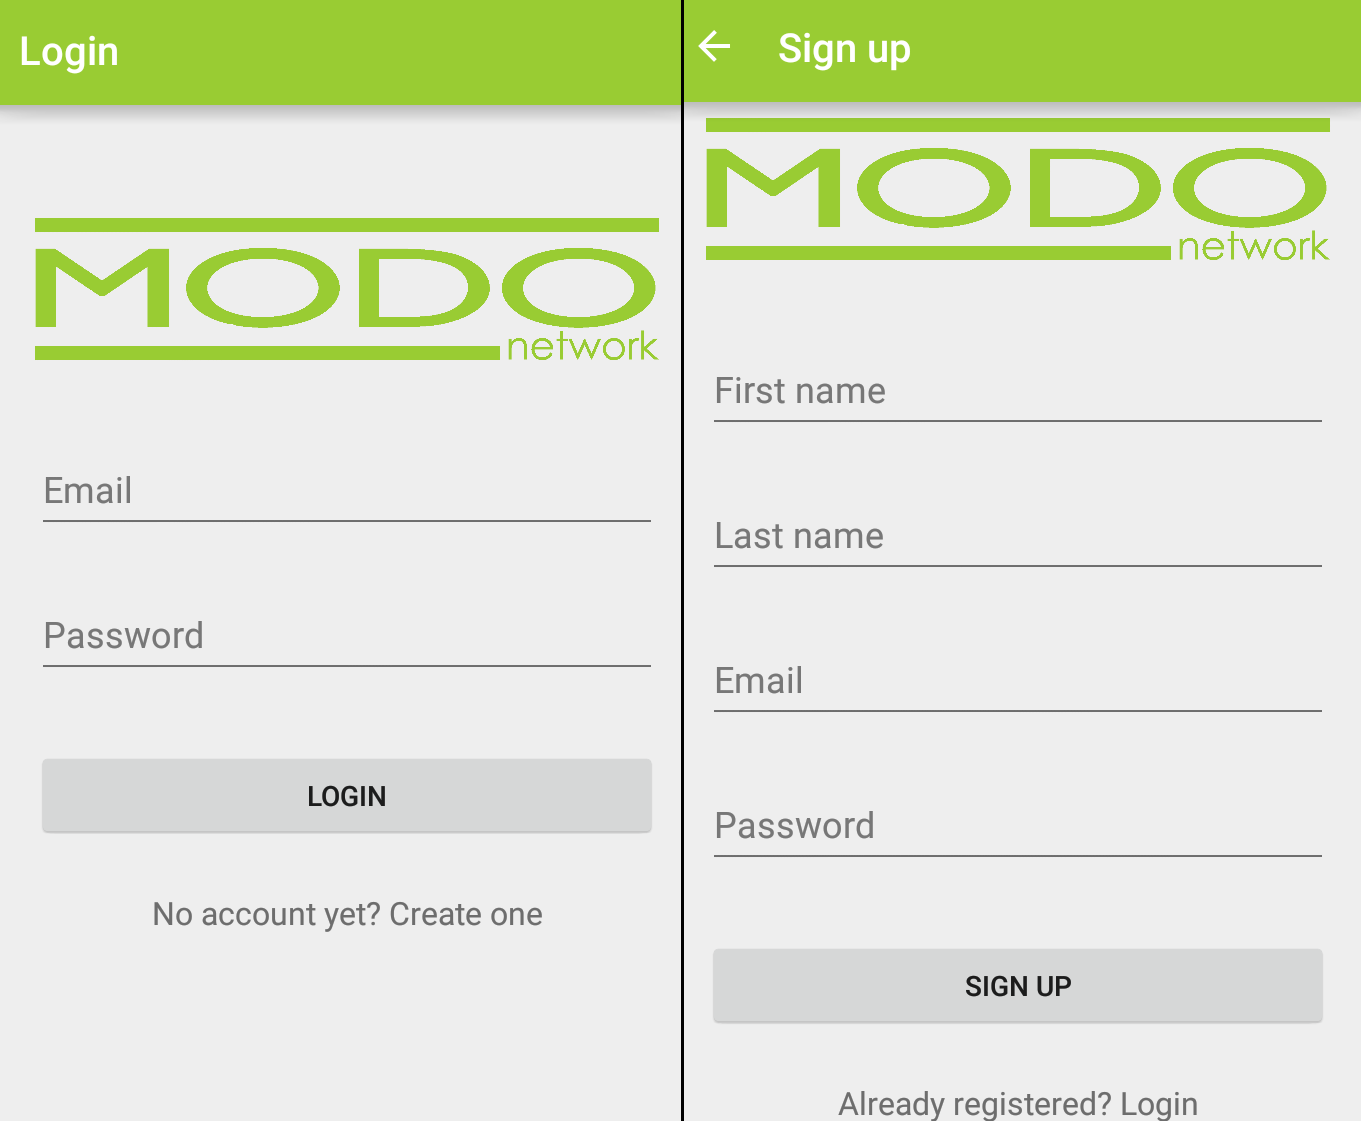
\includegraphics[scale=0.1]{images/prodotto_finale/loginSignUp}
			\caption{Pagine di login e registrazione}
	\end{figure}
	Le pagine per l'autenticazione e per la registrazione presentano dei box di testo per inserire i campi dati richiesti al di sotto di una immagine. I campi dati richiesti dalla pagina per il login sono:
	\begin{itemize}
		\item email;
		\item password.
	\end{itemize}
	A questi la pagina di registrazione aggiunge i campi:
	\begin{itemize}
		\item nome;
		\item cognome.
	\end{itemize}
	Sotto il bottone di conferma è presente un link per passare da una pagina all'altra. Il link per passare dalla pagina di autenticazione alla pagina di registrazione può essere disattivato e nascosto tramite il file di configurazione.

	\newpage
	\subsection{Home page}
	\begin{figure}[H]
		\centering
		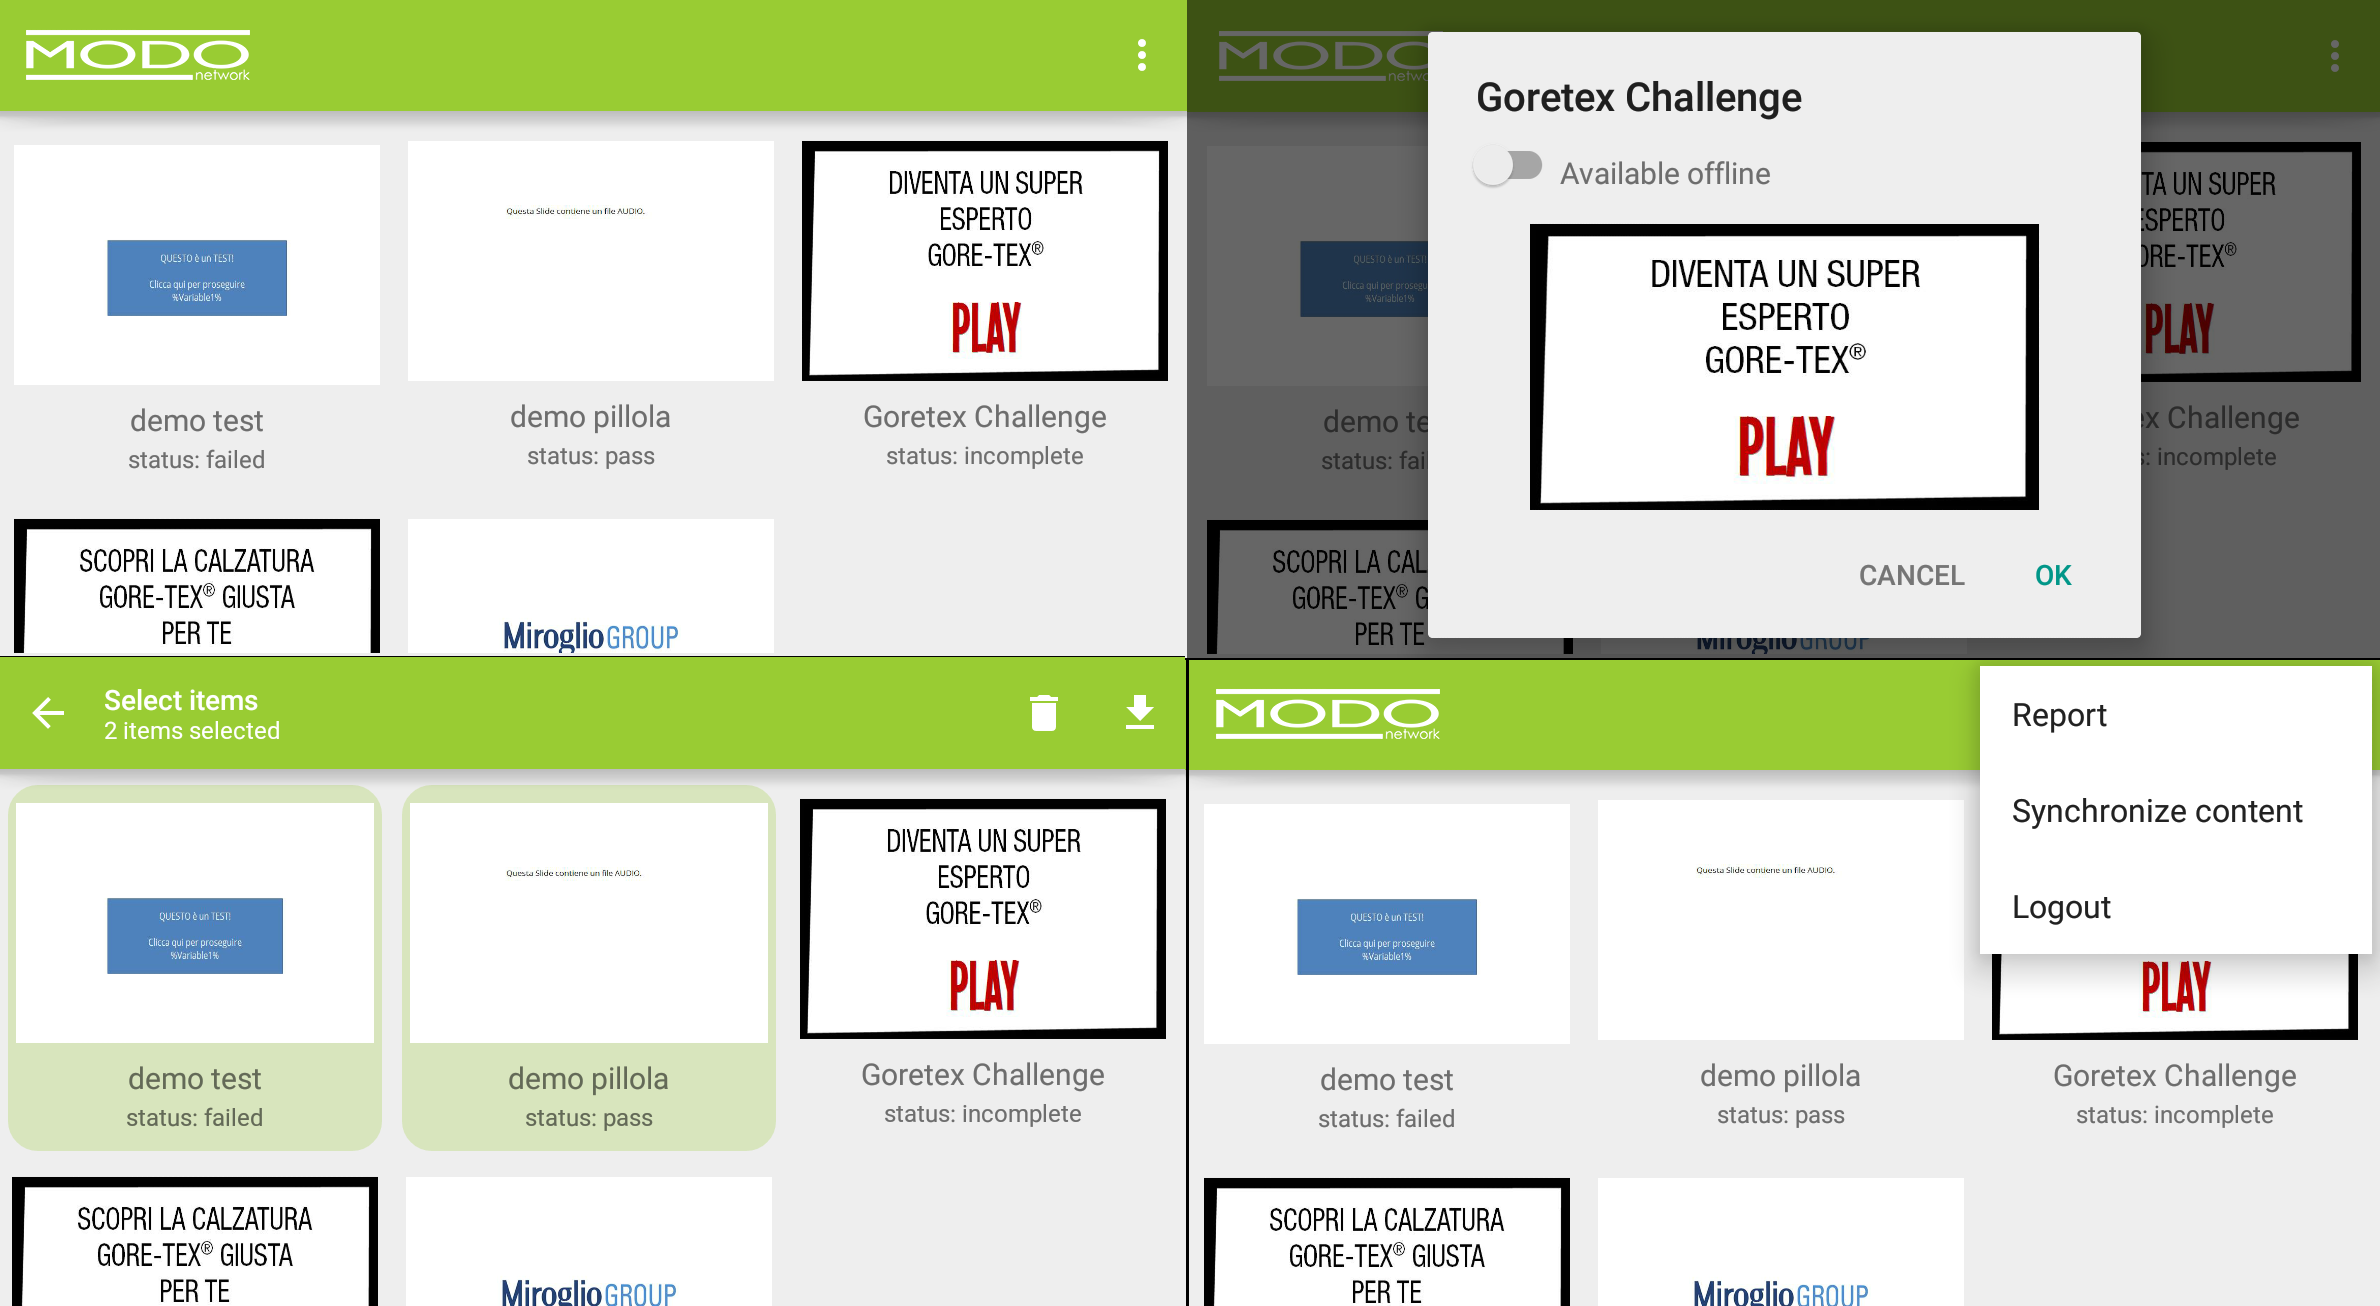
\includegraphics[scale=0.1]{images/prodotto_finale/homex4}
			\caption{Esempio di home page}
	\end{figure}
	L'home page del sito presenta tutti i contenuti a cui un utente può accedere, utilizzando una disposizione a griglia. Effettuando un tap su di un contenuto è possibile visualizzare un pop-up che permette di avviare il corso oppure di effettuarne il download per fruirlo in modalità offline. Tenendo premuto su di un contenuto è possibile selezionarlo. Tale funzionalità permette di effettuare il download di più contenuti in sequenza o di cancellare i corsi selezionati. Infine tale pagina presenta un menù che permette di:
	\begin{itemize}
		\item accedere alla pagina con i report di fruizione;
		\item ripristinare i corsi cancellati;
		\item effettuare il logout.
	\end{itemize}

	\newpage
	\subsection{Pagina con i report}
	\begin{figure}[H]
		\centering
		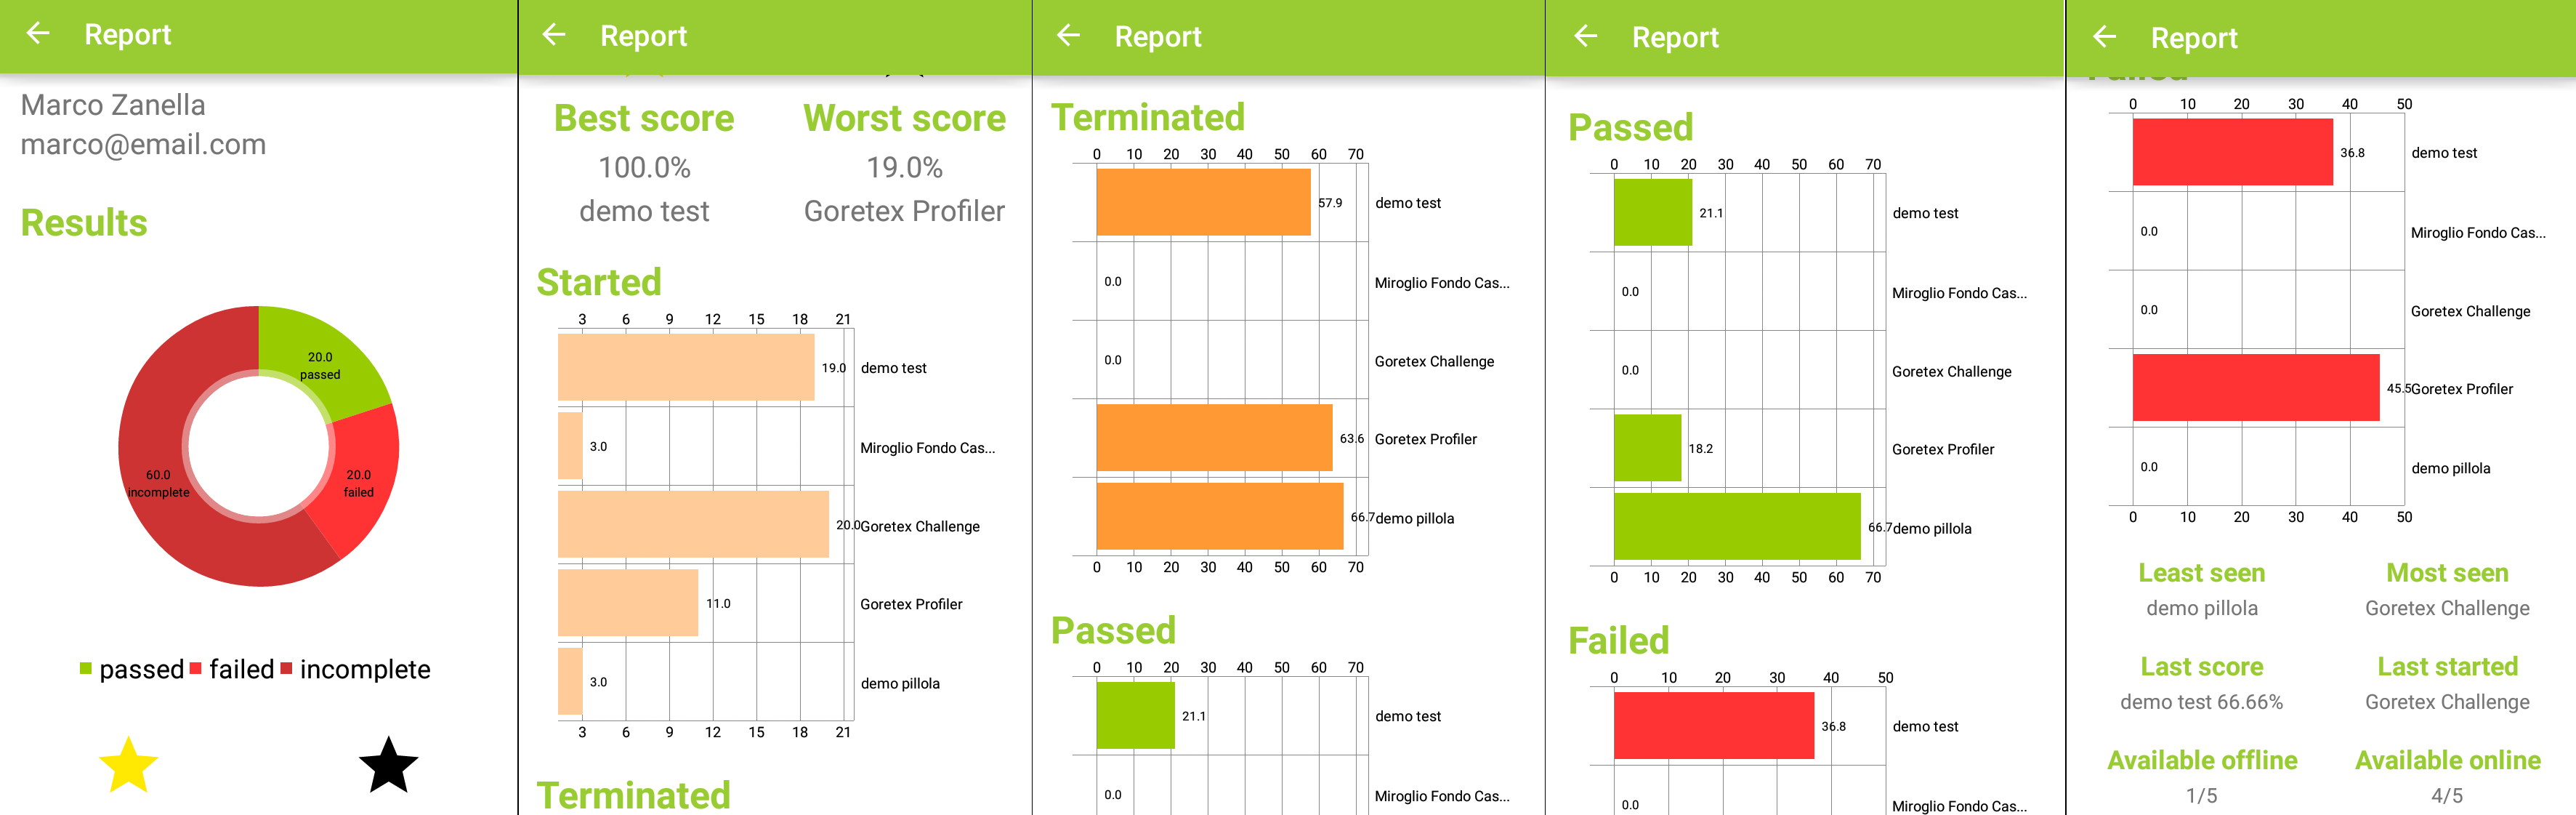
\includegraphics[scale=0.1]{images/prodotto_finale/report_tot}
			\caption{Esempio di pagina con i report}
	\end{figure}
	La pagina con i report di fruizione di un utente mostra alcune statistiche riguardanti i corsi. Nell'ordine tale pagina mostra:
	\begin{itemize}
		\item un grafico a torta che può avere al massimo 4 fette, che rappresentano rispettivamente:
			\begin{itemize}
				\item la percentuale di corsi completati con successo;
				\item la percentuale di corsi completati senza successo;
				\item la percentuale di corsi non completati;
				\item la percentuale di corsi non ancora iniziati.
			\end{itemize}
		\item il migliore e peggiore risultato ottenuto;
		\item i grafici con il numero di volte che è stato iniziato, terminato, superato e non superato ogni corso;
		\item il corso iniziato meno volte e quello iniziato più volte;
		\item l'ultimo corso iniziato e l'ultimo terminato, accompagnato dal punteggio ottenuto;
		\item il numero di corsi disponibili e non offline.
	\end{itemize}

	\newpage
	\subsection{Pagina di visualizzazione dei contenuti}
	\begin{figure}[H]
		\centering
		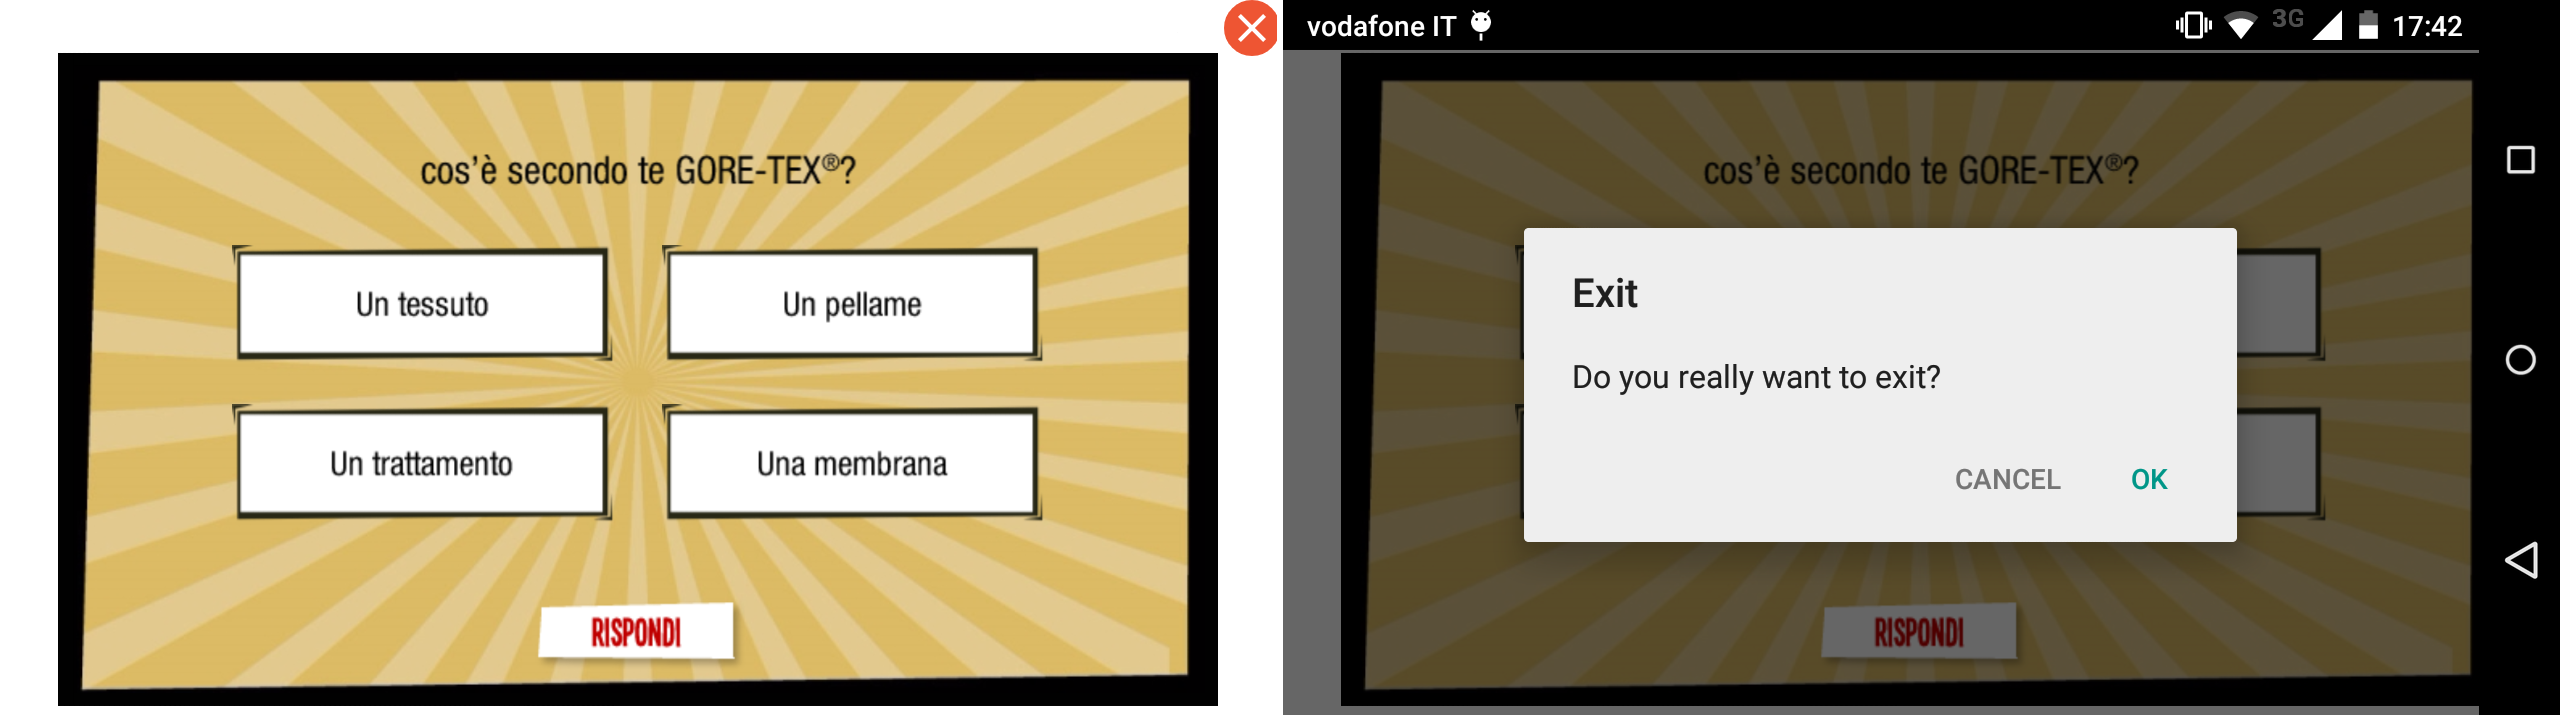
\includegraphics[scale=0.1]{images/prodotto_finale/content_tot}
			\caption{Esempio di riproduzione di un contenuto}
	\end{figure}
	Selezionando un determinato contenuto l'applicazione provvede alla riproduzione del corso. Tale pagina è mostrata in full screen in modo da dare più spazio possibile al contenuto. Per uscire dalla riproduzione è possibile utilizzare il tasto back(per visualizzarlo è necessario prima fare uno swipe verso il basso) oppure il tasto rosso in alto a destra.